\title{Continuum Stewart-Gough Dynamics}
\author{John Till}
\date{}

\documentclass[12pt]{article}

\usepackage[a4paper, margin=0.75in]{geometry}
\usepackage[colorlinks=true,urlcolor=blue]{hyperref}
\usepackage{amsmath,amssymb}
\usepackage{graphicx}

\usepackage{xcolor}
\definecolor{OffWhite}{rgb}{0.93,0.93,0.93}
\definecolor{QtCommentColor}{rgb}{0,0.5,0}
\definecolor{QtKeywordColor}{rgb}{0.5,0.5,0}
\definecolor{QtPurpleColor}{rgb}{0.5,0,0.5}
\definecolor{QtGlobal}{rgb}{0.808,0.361,0}
\definecolor{QtFunctionColor}{rgb}{0,0.404,0.486}
\definecolor{BlenderPythonString}{rgb}{0.392,0,0}
\definecolor{BlenderPythonKeyword}{rgb}{0.502,0,0.314}
\definecolor{BlenderPythonGold}{rgb}{0.373,0.373,0}
\definecolor{BlenderPythonLiteral}{rgb}{0,0,0.784}
\definecolor{BlenderPythonBackground}{rgb}{0.6,0.6,0.6}

\usepackage[T1]{fontenc} %for upquotes in listings
\usepackage{textcomp} %for upquotes in listings
\usepackage{listings}
\lstset{
		language=C++,
		escapeinside={!-}{-!},
		upquote=true,
		%
		otherkeywords={Vector3d, DiagonalMatrix, VectorXd, Matrix3d, Map, MatrixXd, TimeManagerBdfAlpha, 
		              Vector6d, std, fstream,
									UnitX, pow, inverse, transposeMultiply, segment, data, UnitZ, cross, hat_postmultiply,
									Zero, Identity, UnitY, cosseratRodOde, cosseratRodPDE, ode4, col, row, main, plot,
									solveLevenbergMarquardt, Ones, linear_rotation_error, transpose, generateRotation,
									TimeBdfAlpha_SpaceEuler, euler, objFunc, block, clock, advanceTime, endl,
									playAnimation, getC0, obj, initialize_StewartGough_pattern, resize, close},
    morekeywords=[2]{Vector3d, DiagonalMatrix, VectorXd, Matrix3d, Map, MatrixXd, TimeManagerBdfAlpha, 
		                 Vector6d, std, fstream},
		morekeywords=[3]{UnitX, UnitZ, pow, inverse, transposeMultiply, segment, data, cross, hat_postmultiply,
		                 Zero, Identity, UnitY, cosseratRodOde, cosseratRodPDE, ode4, col, row, main, plot,
										solveLevenbergMarquardt, Ones, linear_rotation_error, transpose, generateRotation,
										TimeBdfAlpha_SpaceEuler, euler, objFunc, block, clock, advanceTime, endl, 
										playAnimation, getC0, obj, initialize_StewartGough_pattern, resize, close},
    %
		frame = single,
		rulecolor=\color{black},
    tabsize=4, % tab space width
    showstringspaces=false, % don't mark spaces in strings
		%
		basicstyle=\footnotesize,%\color{QtIdentifier},
		backgroundcolor=\color{OffWhite},
    commentstyle=\color{QtCommentColor}, % comment color
    keywordstyle=\color{QtKeywordColor}, % keyword color
		keywordstyle=[2]{\color{QtPurpleColor}},
		keywordstyle=[3]{\color{QtFunctionColor}},
    stringstyle=\color{QtCommentColor} % string color
}

\begin{document}

\makeatletter
\renewcommand{\@maketitle}{
\newpage
\null
\vskip 2em
\begin{center}
{\LARGE \@title \par}
\end{center}
\par
} \makeatother

\maketitle

Simulating the dynamics of a continuum Stewart-Gough (CSG) robot is an extension of the previous examples to solve elastic rod dynamics and to solve the static CSG kinematics. The theoretical development is described in the paper ``Real-Time Dynamics of Soft and Continuum Robots based on Cosserat-Rod Models'', which is in press with IJRR.

\section{Simulation}

In the first part we implement the CSG dynamics in a C++ script. We start by defining the independent parameters:
\begin{lstlisting}
//Independent Parameters
const double E = 207e9;
const double rad = 0.001;
const double rho = 8000;
const Vector3d g = -9.81*Vector3d::UnitZ();
const double scrib_R = 0.087; //radius of the hole pattern
const double alpha1 = 100*pi/180; //major angle of the hole pattern
const double plate_mass = 0.0921;
const DiagonalMatrix<double, 3> plate_mass_moment(1.91e-4, 1.91e-4, 3.82e-4);
const int N = 200; //Number of spatial points
const double dt = 1.0/120.0; //Time step
const double alpha = -0.2; //Parameter for implicit time discretization
const Vector3d p_start(0, 0, 0.5);
const Vector3d p_final(-0.2, 0, 0.5);
const int num_actuated = 300;
const int num_swaying = 300;
\end{lstlisting}
Many of these variables are design parameters for a continuum Stewart-Gough robot. This includes the plate mass and plate inertia since we will consider the rigid-body dynamics of the end effector. After the CSG parameters, we have the BDF-$\alpha$ parameters ``dt'' and ``alpha''. The last four parameters are specific to this simulation. We will solve the CSG inverse kinematics to generate a trajectory for which the quasi-static model begins at ``p\_start'' and moves to ``p\_final''. However, the target points have been chosen so that this trajectory causes elastic instability, and following the trajectory using the CSG forward dynamics model will cause the robot to snap. The number of time steps spent following the input trajectory is ``num\_actuated'', and ``num\_swaying'' is the number of time steps to continue simulating after the actuator values no longer change.

\newpage \noindent
With the independent parameters taken care of, we have various dependent parameters which may be calculated:
\begin{lstlisting}
//Dependent parameter calculations
const double c0 = TimeManagerBdfAlpha::getC0(dt,alpha);
const double G = E/(2*(1+0.3));
const double A = pi*pow(rad,2);
const double I = pi*pow(rad,4)/4;
static Vector3d pE = p_start;
static Matrix3d RE = Matrix3d::Identity();
const double alpha2 = 120*pi/180 - alpha1; //minor angle of the hole pattern
const DiagonalMatrix<double, 3> Kse_inv =
    DiagonalMatrix<double, 3>(G*A,G*A,E*A).inverse();
const DiagonalMatrix<double, 3> Kbt_inv =
    DiagonalMatrix<double, 3>(E*I,E*I,G*2*I).inverse();
const DiagonalMatrix<double, 3> rhoJ = rho*DiagonalMatrix<double, 3>(I, I, 2*I);
const double rhoA = rho*A;
const Vector3d rhoAg = rho*A*g;
static Vector6d L;
\end{lstlisting}
The forward problem (kinematic or dynamic) is to solve for ``pE'' and ``RE'' given the leg lengths ``L'', and the inverse problem is to solve for ``L'' given ``pE'' and ``RE''. These variables are declared static since they will change throughout the simulation, while the other parameters are declared constant.

The script has a function to setup the CSG hole pattern as in the static CSG BVP and functions for the ODE and PDE as in the dynamic rod problem. These are fundamentally unchanged, so we won't consider them in detail here. Compared to the dynamic rod problem, the CSG requires several more state and dynamic variables:
\begin{lstlisting}
static MatrixXd Y[6], Z[6], Z_h[6];
static MatrixXd X(24,1), X_h(24,1);
const Map<Vector3d> pE_h(&X_h(0,0));
const Map<Vector3d> vE_h(&X_h(3,0));
const Map<Matrix3d> RE_h(&X_h(6,0));
const Map<Vector3d> wE_h(&X_h(15,0));
const Map<Vector6d> L_h(&X_h(18,0));
\end{lstlisting}
We have states ``Y'' and dynamic variables ``Z'' for each rod. We also have several dynamic variables not associated with the rods. We lump these into a variable ``X'', and then create maps to reference the meaningful components of X.

Since there are strong similarities in the inverse kinematics, forward kinematics, and forward dynamics objective functions, we combine them all into a single templated function. We begin this function by addressing the dissimilarities in the guess:
\begin{lstlisting}
template<bool is_forward, bool is_dynamic>
VectorXd obj(VectorXd guess){
    VectorXd residual(42);

    if(is_forward){
        pE = guess.segment<3>(36);
        RE = generateRotation(guess.segment<3>(39));
    }else{
        L = guess.segment<6>(36);
    }
\end{lstlisting}
For this simulation we consider a robot with the rods fully attached so that they support torsion and cannot spin, which results in a 42x42 system of nonlinear equations. The last six elements of the guess are the leg lengths for the inverse problem, and in the forward problem the last six elements are used to generate the end-effector pose. The ``generateRotation'' function uses Rodrigues' rotation formula to generate a rotation matrix from a 3x1 vector.

In the next step we solve for the dynamic movement of the end effector and create variables to sum the error in the plate's rigid body dynamics:
\begin{lstlisting}
    Matrix3d Jg = RE*plate_mass_moment*RE.transpose();
    Vector3d vE, wE, EF, EM;
    Vector6d L_t;
    if(is_dynamic){
        vE = c0*pE + pE_h;
        Vector3d aE = c0*vE + vE_h;
        wE = inv_hat((c0*RE+RE_h)*RE.transpose());
        Vector3d wE_t = c0*wE + wE_h;
        L_t = c0*L + L_h;

        EF = plate_mass*(g - aE);
        EM = -Jg*wE_t - wE.cross(Jg*wE);
    }else{
        vE = wE = Vector3d::Zero();
        L_t = Vector6d::Zero();

        EF = plate_mass*g;
        EM = Vector3d::Zero();
    }
    X << pE, vE, Map<VectorXd>(RE.data(), 9), wE, L;
\end{lstlisting}
If we are considering dynamic behavior, the force and moment equilibrium errors ``EF'' and ``EM'' will include inertial effects from the plate mass. In both cases we set ``X'' so that we can track its history.

Finally we can integrate the rods and finish calculating the residual:
\begin{lstlisting}
    for(int i = 0; i < 6; i++){
        Vector3d n0 = guess.segment<3>(6*i);
        Vector3d m0 = guess.segment<3>(6*i+3);
        double wz0 = 0; //Assume negligible torsional velocity through baseplate
        VectorXd y0(24);
        y0 << p0[i], 1, 0, 0, 0, 1, 0, 0, 0, 1, n0, m0, 0, 0, L_t(i), 0, 0, wz0;
        Y[i].col(0) = y0;

        //Numerically integrate the Cosserat rod equations
        if(is_dynamic) TimeBdfAlpha_SpaceEuler<cosseratRodPDE,24,12,N>
                                              (Y[i],Z[i],y0,L(i),Z_h[i]);
        else euler<cosseratRodOde,24,12,N>(Y[i],Z[i],y0,L(i));

        Vector3d pL_shot = Y[i].block<3,1>(0, N-1);
        Matrix3d RL_shot = Map<Matrix3d>(Y[i].block<9,1>(3, N-1).data());
        Vector3d nL = Y[i].block<3,1>(12, N-1);
        Vector3d mL = Y[i].block<3,1>(15, N-1);

        residual.segment<3>(6*i) = pL_shot - (pE + RE*r[i]);
        residual.segment<3>(6*i+3) = linear_rotation_error(RL_shot,RE);

        EF -= nL;
        EM -= (mL + (RE*r[i]).cross(nL));
    }
    residual.segment<3>(36) = EF;
    residual.segment<3>(39) = EM;
		
    return residual;
}
\end{lstlisting}
The only variability in the approach is whether we integrate using a static or dynamic method. In all cases, we integrate a rod, calculate the geometric errors, and continue summing the equilibrium errors until we have the full residual vector.

With the objective function finished, we have all the subfunctions we need and we can move on to the main method. Of course we begin by setting up the hole pattern:
\begin{lstlisting}
int main(int, char**){
    initialize_StewartGough_pattern();
\end{lstlisting}
Calling the forward dynamic objective function with ``obj<true,true>'' is not very intuitive, but we can fix this by defining several Booleans:
\begin{lstlisting}
const bool Kinematics = false;
const bool Dynamics = true;
const bool Forward = true;
const bool Inverse = false;
\end{lstlisting}
This allows us to refer to the forward dynamics function as ``obj<Forward,Dynamics>'' and the inverse kinematics as ``obj<Inverse,Kinematics>''.

When we declared the arrays for the rod variables, it was not convenient to initialize their sizes in the declaration. We set the sizes of these variables here:
\begin{lstlisting}
//Setup the grid
for(int i = 0; i < 6; i++){
    Y[i].resize(24,N);
    Z[i].resize(12,N);
    Z_h[i].resize(12,N);
}
\end{lstlisting}
Now we have done the setup to actually start simulating. The first half of the simulation is the inverse kinematics problem of solving the motor inputs to realize the trajectory:
\begin{lstlisting}
//Solve the "home" configuration
VectorXd guess(42);
guess << VectorXd::Zero(36), pE(2)*VectorXd::Ones(6);
guess = solveLevenbergMarquardt<obj<Inverse,Kinematics> >(guess);

//Declare actuation profile and set first entry
Vector6d leg_lengths[num_actuated+1];
leg_lengths[0] = guess.segment<6>(36);

//Inverse kinematics to find the input trajectory
for(int i = 1; i <= num_actuated; i++){
    std::cout << "IK: " << i << std::endl;

    pE = p_start + (p_final - p_start)*i/static_cast<double>(num_actuated);
    guess = solveLevenbergMarquardt<obj<Inverse,Kinematics> >(guess);
    leg_lengths[i] = guess.segment<6>(36);
}
\end{lstlisting}
We linearly interpolate between the start and final points. Solved values are stored in our ``leg\_lengths'' array.

\newpage \noindent
Now we move on to the second half of the simulation: the forward dynamics. We need to use a few lines to declare variables and set up the ICs:
\begin{lstlisting}
//Reset the robot state and solve ICs
pE = p_start;
L = leg_lengths[0];
guess << VectorXd::Zero(36), p_start, Vector3d::Zero();
guess = solveLevenbergMarquardt<obj<Forward,Kinematics> >(guess);

//Prepare for the dynamic problem
int total_frames = 1 + num_actuated + num_swaying;
MatrixXd centerlines(6*3*total_frames,N), g_frames(3*total_frames,4);
VectorXd pEx(total_frames), pEz(total_frames);
TimeManagerBdfAlpha* time_scheme[7];
for(int i = 0; i < 6; i++)
    time_scheme[i] = new TimeManagerBdfAlpha(Z[i], Z_h[i], dt, alpha);
time_scheme[6] = new TimeManagerBdfAlpha(X, X_h, dt, alpha);
\end{lstlisting}
The guess is reset, and the last six elements will represent the pose now. We solve the forward kinematics problem to reset the robot to the starting position, and we get ready to calculate time derivatives using our time manager abstraction. We create four variables, ``centerlines'', ``g\_frames'', ``pEx'', and ``pEz'', which we will use to store the simulation results.

Now we have the dynamic simulation loop:
\begin{lstlisting}
//Simulate the dynamic behavior
for(int i = 0; i < total_frames; i++){
    std::cout << "Dynamic: " << i << std::endl;

    if(i <= num_actuated) L = leg_lengths[i];
    guess = solveLevenbergMarquardt<obj<Forward,Dynamics> >(guess);
    for(int j = 0; j < 7; j++) time_scheme[j]->advanceTime();

    pEx(i) = pE.!-\textcolor{QtFunctionColor}{x}-!();
    pEz(i) = pE.!-\textcolor{QtFunctionColor}{z}-!();
    g_frames.block<3,3>(3*i,0) = RE;
    g_frames.block<3,1>(3*i,3) = pE;
    for(int j = 0; j < 6; j++)
        centerlines.block<3,N>(18*i+3*j,0) = Y[j].block<3,N>(0,0);
}
\end{lstlisting}
For each time step we set the leg lengths based on the input motion profile we solved earlier, then we solve the forward dynamics problem and calculate dynamic terms for the next step. The last six lines of the loop are used to store simulation results. In the final lines after the dynamic loop, we save the data to a couple files and plot the dynamic tip trajectory:
\begin{lstlisting}
//Save results for Blender visualization
std::fstream file("centerlines.dat", std::fstream::out);
file << centerlines;
file.close();

file = std::fstream("ee_transformations.dat", std::fstream::out);
file << g_frames;
file.close();

//Show the end-effector trajectory
#ifdef QT_CORE_LIB
plot(pEx, pEz, "CSG Dynamic Trajectory", "x (m)", "z (m)");
#endif
\end{lstlisting}
Running the program causes a graph of the end-effector trajectory to popup:
\begin{figure}[h]
	\centering
		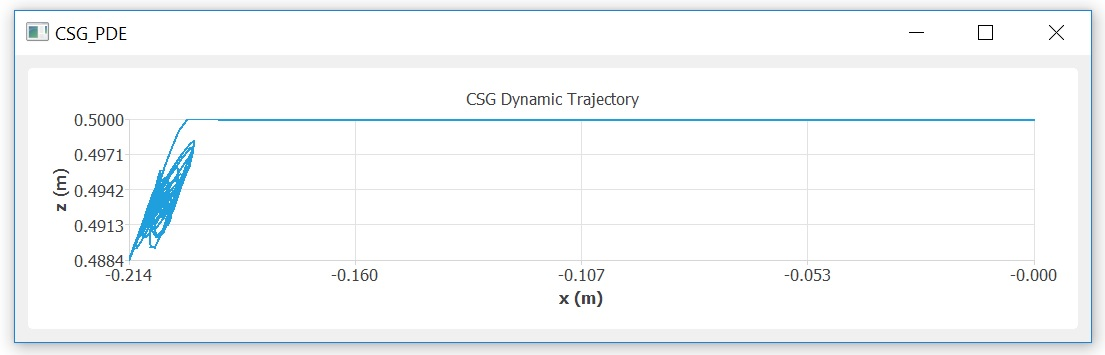
\includegraphics[width=0.9\textwidth]{fig/SolutionPlot.jpg}
	\label{fig:SolutionPlot}
\end{figure}

\noindent The largest saved file contains all six rod centerlines at every time step, and the smaller file contains the end-effector position and rotation at each time step. We could visualize this data using Qt, but to keep this simulation script short and to make a shiny video in Blender, we'll handle visualization in a second part.

The program takes some time to run. With enough effort we could make the simulation run in soft real-time by writing a user-supplied Jacobian function, piddling with the hot-loop in the integration routine, and multithreading. However, the current simulation script is almost 300 lines, and we've already seen how to make all those changes, so we won't incorporate those changes here.

\section{Visualization}

One of the nice features of Blender is that in addition to using the user interface, you can also perform modeling tasks using Python scripts. This is perfect for generating 3d models from simulation results.

The simulation output files ``centerlines.dat'' and ``ee\_transformations.dat'' should be moved to the ``Blender'' subfolder. This task isn't automated since the directory in which the simulation output files are generated will depend on how the C++ code is run. If run with Qt, the output files should be in the build folder. Once these files are moved, the Blender script is ready to run.

Upon opening the ``CSG\_Animation.blend'' file, the Python scripting pane will be in the upper left. There is a ``Run Script'' button on the bottom right of the pane as shown below:
\begin{figure}[h]
	\centering
		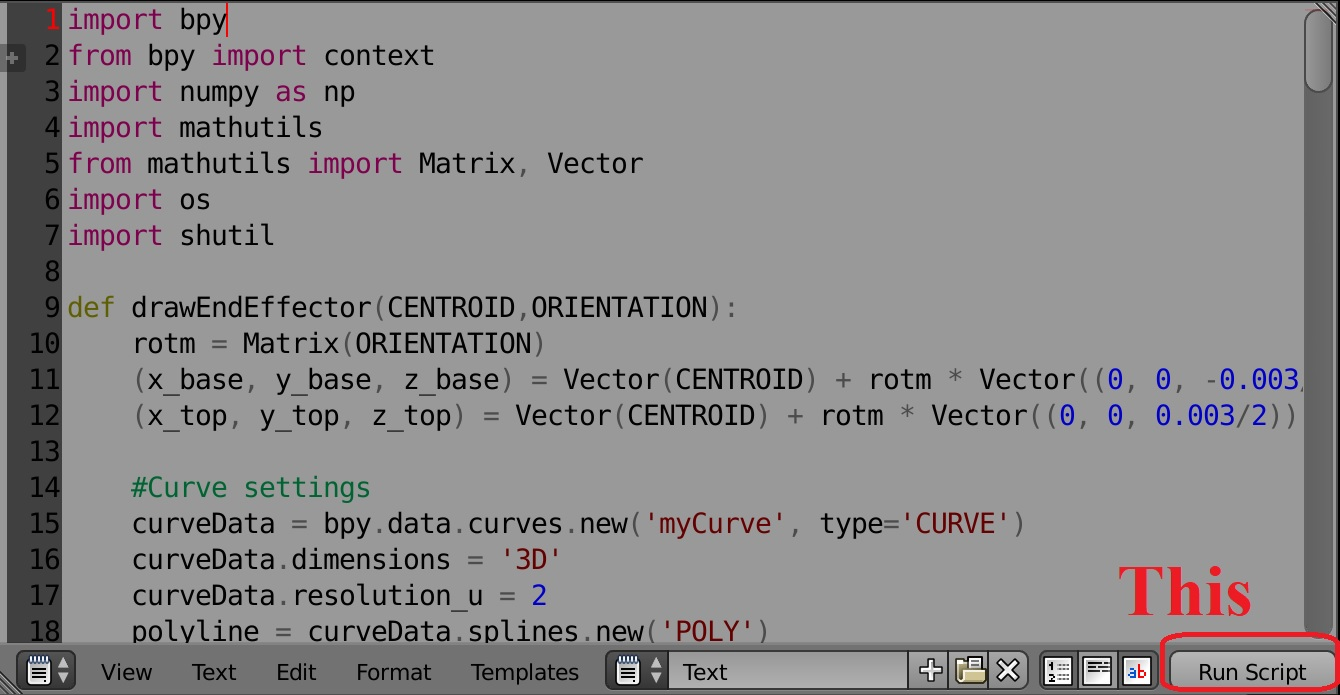
\includegraphics[width=0.95\textwidth]{fig/ScriptingPane.jpg}
	\label{fig:Pane}
\end{figure}

\noindent I recommend using ``Window $\rightarrow$ Toggle System Console'' prior to running a script because this will show the output and allow you to stop a running script by hitting ``Ctrl+C'' with the console selected.

\lstset{
		language=Python,
		escapeinside={!-}{-!},
		%
		deletekeywords={def, type, object, range, len, int},
		otherkeywords={def, True, False, type, object, range, len},
		morekeywords=[2]{def},
		morekeywords=[3]{True, False, type, object, range, len},
		%
		frame = single,
		rulecolor=\color{black},
    tabsize=4, % tab space width
    showstringspaces=false, % don't mark spaces in strings
		%
		basicstyle=\footnotesize,%\color{QtIdentifier},
		%backgroundcolor=\color{BlenderPythonBackground},
    %commentstyle=\color{QtCommentColor}, % comment color
    keywordstyle=\color{BlenderPythonKeyword}, % keyword color
		keywordstyle=[2]{\color{BlenderPythonGold}},
		keywordstyle=[3]{\color{BlenderPythonLiteral}},
    stringstyle=\color{BlenderPythonString}, % string color
		literate={0}{{\textcolor{BlenderPythonLiteral}{0}}}{1}%
             {1}{{\textcolor{BlenderPythonLiteral}{1}}}{1}%
             {2}{{\textcolor{BlenderPythonLiteral}{2}}}{1}%
             {3}{{\textcolor{BlenderPythonLiteral}{3}}}{1}%
             {4}{{\textcolor{BlenderPythonLiteral}{4}}}{1}%
             {5}{{\textcolor{BlenderPythonLiteral}{5}}}{1}%
             {6}{{\textcolor{BlenderPythonLiteral}{6}}}{1}%
             {7}{{\textcolor{BlenderPythonLiteral}{7}}}{1}%
             {8}{{\textcolor{BlenderPythonLiteral}{8}}}{1}%
             {9}{{\textcolor{BlenderPythonLiteral}{9}}}{1}%
             {.0}{{\textcolor{BlenderPythonLiteral}{.0}}}{2}% Following is to ensure that only periods
             {.1}{{\textcolor{BlenderPythonLiteral}{.1}}}{2}% followed by a digit are changed.
             {.2}{{\textcolor{BlenderPythonLiteral}{.2}}}{2}%
             {.3}{{\textcolor{BlenderPythonLiteral}{.3}}}{2}%
             {.4}{{\textcolor{BlenderPythonLiteral}{.4}}}{2}%
             {.5}{{\textcolor{BlenderPythonLiteral}{.5}}}{2}%
             {.6}{{\textcolor{BlenderPythonLiteral}{.6}}}{2}%
             {.7}{{\textcolor{BlenderPythonLiteral}{.7}}}{2}%
             {.8}{{\textcolor{BlenderPythonLiteral}{.8}}}{2}%
             {.9}{{\textcolor{BlenderPythonLiteral}{.9}}}{2}%
						 {type}{type}{4}%
						 {object}{object}{6}%
						 {range}{range}{5}%
						 {len}{len}{3}%
						 {int}{int}{3}%
						 {format}{format}{6}%
}

This script has two parts. First, it creates a JPEG image of the robot for each time step of the simulation. For each frame it loops through the rod centerlines and uses a helper function ``drawRod'' to create the rod shape. It also reads the end-effector pose and draws a transparent plate using the ``drawEndEffector'' function. Then the script renders the scene and saves a JPEG before deleting everything to start on the next frame.
\begin{figure}[h]
	\centering
		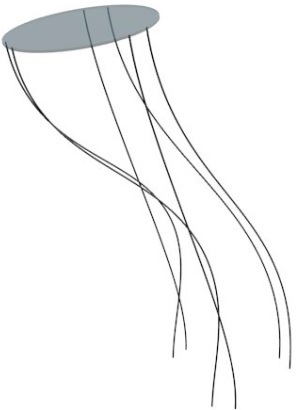
\includegraphics[width=0.3\textwidth]{fig/Render.jpg}
	\label{fig:Render}
\end{figure}

In the second part, the script stitches the frames together into an AVI movie of the simulation using Blender's ``sequencer''. The movie is generated in the subfolder ``Blender/output''. The resolution of 480x240 is rather low, but this greatly decreases the file sizes and time to run the script compared to a 1080p movie.

A detailed explanation of the script is a bit tangential, and besides that I am not quite confident enough in my Blender or Python skills to discuss the code at length. But the basic elements of what we need to visualize continuum robots are present, and using this for other rod elasticity problems would require minor adaptations. The script is given here:

\begin{lstlisting}
import bpy
from bpy import context
import numpy as np
import mathutils
from mathutils import Matrix, Vector
import os
import shutil

def drawEndEffector(p,R):
    rotm = Matrix(R)
    (x_base, y_base, z_base) = Vector(p) + rotm * Vector((0, 0, -0.003/2))
    (x_top, y_top, z_top) = Vector(p) + rotm * Vector((0, 0, 0.003/2))
    	
    #Curve settings
    curveData = bpy.data.curves.new('myCurve', type='CURVE')
    curveData.dimensions = '!-\textcolor{BlenderPythonString}{3D}-!'
    curveData.resolution_u = 2
    polyline = curveData.splines.new('POLY')
    polyline.points.add(1)
    polyline.points[0].co = (x_base, y_base, z_base, 1)
    polyline.points[1].co = (x_top, y_top, z_top, 1)

    cross_section = bpy.ops.curve.primitive_bezier_circle_add(radius=0.091)
    ob = bpy.context.object
    ob.name = 'cross_section_ee'

    curveOB = bpy.data.objects.new('myCurve', curveData)
    scn = bpy.context.scene
    scn.objects.link(curveOB)
    scn.objects.active = curveOB
    curveOB.select = True
    curveOB.data.bevel_object = bpy.data.objects['cross_section_ee']
    curveOB.data.use_fill_caps = True
    
    mat = bpy.data.materials.new("RGBA")
    mat.use_transparency = True;
    mat.diffuse_color = (117/255.0, 214/255.0, 1)
    mat.alpha = 0.5;
    curveOB.active_material = mat

def drawRod(p):
    (rows,cols) = p.shape

    #Curve settings
    curveData = bpy.data.curves.new('tCurve', type='CURVE')
    curveData.dimensions = '!-\textcolor{BlenderPythonString}{3D}-!'
    curveData.resolution_u = 2
    polyline = curveData.splines.new('POLY')
    polyline.points.add(cols-1)
        
    cross_section = bpy.ops.curve.primitive_bezier_circle_add(radius=0.001)
    ob = bpy.context.object
    ob.name = 'tcross_section'

    #Loop through spatial steps
    for i in range(0,cols):
    	x,y,z = p[0,i], p[1,i], p[2,i]
    	polyline.points[i].co = (x, y, z, 1)
            
    curveOB = bpy.data.objects.new('myCurve', curveData)
    scn = bpy.context.scene
    scn.objects.link(curveOB)
    scn.objects.active = curveOB
    curveOB.select = True
    curveOB.data.bevel_object = bpy.data.objects['tcross_section']
    curveOB.data.use_fill_caps = True
    
### MAIN ###
script_dir = os.getcwd() #<-- absolute path of dir the script is in
bpy.context.scene.world.horizon_color = (1,1,1) #white background
bpy.data.scenes["Scene"].render.image_settings.file_format = 'JPEG'
bpy.data.scenes["Scene"].render.use_sequencer = False
scene = bpy.data.scenes["Scene"]
scene.render.resolution_x = 480*2
scene.render.resolution_y = 240*2

#Load data
centerline_data = np.loadtxt( os.path.join(script_dir, 'centerlines.dat'))
ee_data = np.loadtxt( os.path.join(script_dir, 'ee_transformations.dat'))
(rows,cols) = centerline_data.shape
total_frames = int(rows/18);

#Loop through time steps to create frames
for i in range(0,total_frames):
    ee_pos = ee_data[3*i:3*i+3, 3];
    ee_rot = ee_data[3*i:3*i+3, 0:3];
    drawEndEffector(ee_pos, ee_rot);
    for j in range(0,6):
        p = centerline_data[ 18*i+3*j:18*i+3*j+3, 0:cols ];
        drawRod(p)

    rel_path = 'temp/frame_' + format(i, '!-\textcolor{BlenderPythonString}{05d}-!') + '.jpg'
    abs_file_path = os.path.join(script_dir, rel_path)
    bpy.data.scenes["Scene"].render.filepath = abs_file_path
    bpy.ops.render.render( animation=False, write_still=True )
    
    for item in bpy.data.objects:
        if item.type == 'MESH' or item.type=='CURVE':
            item.select = True
            bpy.ops.object.delete() #clear all objects for next frame

#Setup video creation
bpy.data.scenes["Scene"].render.use_sequencer = True
area = bpy.context.area
old_type = area.type
area.type = 'SEQUENCE_EDITOR'
imdir = os.path.join(script_dir, 'temp')
filelist = [{"name":i} for i in os.listdir(imdir)]
n = len(filelist)

#Create the video from frames
a = bpy.ops.sequencer.image_strip_add(
    directory = imdir, files = filelist, channel=1, frame_start=0, frame_end=n-1
    )
out_dir = os.path.join(script_dir, 'output', 'CSG_Dynamics.avi')
stripname=filelist[0].get("name");
bpy.data.scenes["Scene"].frame_end = n
bpy.data.scenes["Scene"].render.image_settings.file_format = 'AVI_JPEG'
bpy.data.scenes["Scene"].render.filepath = out_dir 
bpy.ops.render.render( animation=True )

#Cleanup
area.type = old_type
rel_path = 'temp'
abs_file_path = os.path.join(script_dir, rel_path)
shutil.rmtree(abs_file_path)
\end{lstlisting}

\end{document}